\documentclass[a4paper]{article}
\usepackage[margin=1.25in]{geometry}
\usepackage{bookmark}

\usepackage{tabularx}
\newcolumntype{L}{>{\centering\arraybackslash}X}

\usepackage{enumitem}
\renewcommand\labelitemi{\textbf{\textendash}}

\usepackage[dvipsnames]{xcolor}
\definecolor{emerald}{RGB}{2,138,15}

\usepackage{hyperref}
\hypersetup{
    colorlinks,
    linkcolor={black},
    citecolor={blue!50!black},
    urlcolor={blue!65!black}
}

\usepackage{fancyvrb}
\fvset{frame=single, vspace=1.5em, commandchars=\\\{\}}

\usepackage[skins]{tcolorbox}
\newtcolorbox{boxx}[2][]{%
  enhanced,colback=white,colframe=black,coltitle=black,
  sharp corners,boxrule=0.75pt,left=5pt,right=0pt,top=0pt,bottom=0pt,
  fonttitle=\ttfamily,
  attach boxed title to top center={yshift=-0.5\baselineskip},
  boxed title style={tile,size=minimal,left=0.5mm,right=0.5mm,
  colback=white,before upper=\strut},
  title=#2,#1
}

\usepackage{listings} 
\lstset{
  basicstyle=\ttfamily,
  breaklines=true,
  escapeinside={/<}{>/},
  moredelim=**[is][\color{red}]{/-}{-/},
  moredelim=**[is][\color{emerald}]{/+}{+/},
  breakindent=0pt,
  columns=fullflexible
}
\lstnewenvironment{code}[1][]{\begin{myframe}{#1}}{\end{myframe}}

\title{CS7.302: Assignment 1}
\author{Himanshu Singh}
\date{\today}

\begin{document}

\maketitle

\section{Camera coordinate system}

The discrepancy stems from the limited range of real numbers the ``float'' data type (used in most of our operations) can represent. A simple change in type definition of \texttt{Vector3f}, from \texttt{Vector3<float>} to \texttt{Vector3<double>} helps consolidate our claim.

A more scalable way to remedy this is to center our coordinates around the camera. This way the primitives that are proximate to the camera are not only more likely to be represented accurately, but remain so after operations like, say a cross product, which can scale up the magnitude of the resulting vector.

The changes made in implementation were as follows:

\begin{boxx}{scene.cpp: Scene::parse(\ldots)}
\begin{lstlisting}
/-- this->camera = Camera(from, to, up, ...) -/
/++ this->camera = Camera(Vector3f(0, 0, 0), to - from, up, ...) +/
/-- auto surf = createSurfaces(...); -/
/++ auto surf = createSurfaces(..., /*cameraCoords=*/ from); +/
\end{lstlisting}
\end{boxx}

\begin{boxx}{surface.cpp: createSurfaces(\ldots)}
\begin{lstlisting}
/-- vertices[v] = Vector3f(vx, vy, vz);-/
/++ vertices[v] = Vector3f(vx, vy, vz) - cameraCoords;+/
\end{lstlisting}
\end{boxx}

\begin{figure}[ht]
  \centering
  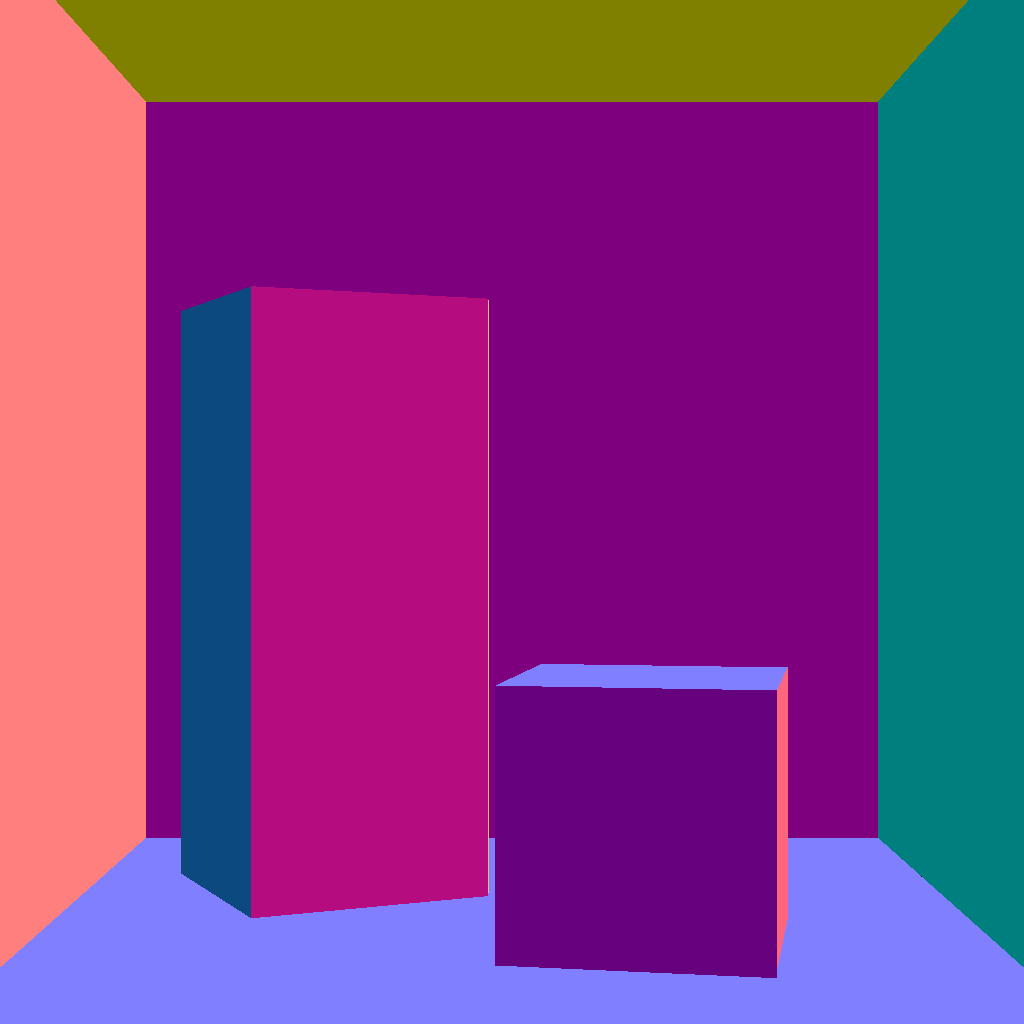
\includegraphics[width=0.4\textwidth]{q1/incorrect.png}
  \caption{Rendering of incorrect.json}
\end{figure}

\section{Acceleration Structure: Bounding Volume Hierarchy}

\subsection{Brief Walkthrough}

\begin{boxx}{render.cpp: main(...)}
\begin{lstlisting}
/++ // initialise structures necessary for the intersection variant
  if (intersectionVariant > 0)
    scene.createBoundingBoxes();
  if (intersectionVariant > 1)
    scene.createBVH();
  if (intersectionVariant > 2)
    scene.createTriangleBVH(); +/
\end{lstlisting}
\end{boxx}

\begin{boxx}{render.h: struct Integrator}
\begin{lstlisting}
/-- long long render; -/
/++ long long render(int intersectionVariant);
  // the renderer now invokes one of the four intersection handlers +/
\end{lstlisting}
\end{boxx}

\begin{boxx}{scene.h: struct Scene}
\begin{lstlisting}
/++ Interaction rayIntersect(Ray& ray);
  // iterates Scene::surfaces, invokes Surface::rayIntersect

  Interaction AABBIntersect(Ray& ray);
  // iterates Scene::boxes, invokes AABB::slabTest

  Interaction BVHIntersect(Ray& ray, int idx);
  // traverses Scene::bvh, invokes AABB::slabTest and Surface::rayIntersect

  Interaction twoLevelBVHIntersect(Ray& ray, int idx);
  // traverses Scene::bvh, invokes AABB::slabTest and Surface::triangleBVHIntersect

  Interaction triangleBVHIntersect(Ray& ray, int surface, int idx);
  // traverses Scene::trianglebvh, AABB::slabTest and invokes Surface::rayTriangleIntersect +/
\end{lstlisting}
\end{boxx}

\subsection{Timings}

\begin{table}[ht]
\centering
\renewcommand{\arraystretch}{1.5}
\begin{tabularx}{\linewidth}{cLLLL}
\hline
& CornellBox (High Polygons) & CornellBox (Low Polygons) & Donuts & TableTop \\
\hline
Na\"ive Intersection & 278423.50 & 66889.09 & 84465.70 & 77964.17 \\
AABB Intersections & 27022.30 & 9431.47 & 12031.77 & 9574.50 \\
BVH on AABB & 27687.43 & 9742.76 & 11976.73 & 9478.07 \\
BVH on Triangles & 737.58 & 725.51 & 1225.93 & 250.76 \\
\hline
\end{tabularx}
\caption{Time taken (in ms) for rendering by various intersection variants}
\end{table}

\pagebreak

\subsection{Rendered Images}

\begin{figure}[htb]
  \begin{minipage}[t]{.4\textwidth}
      \centering
      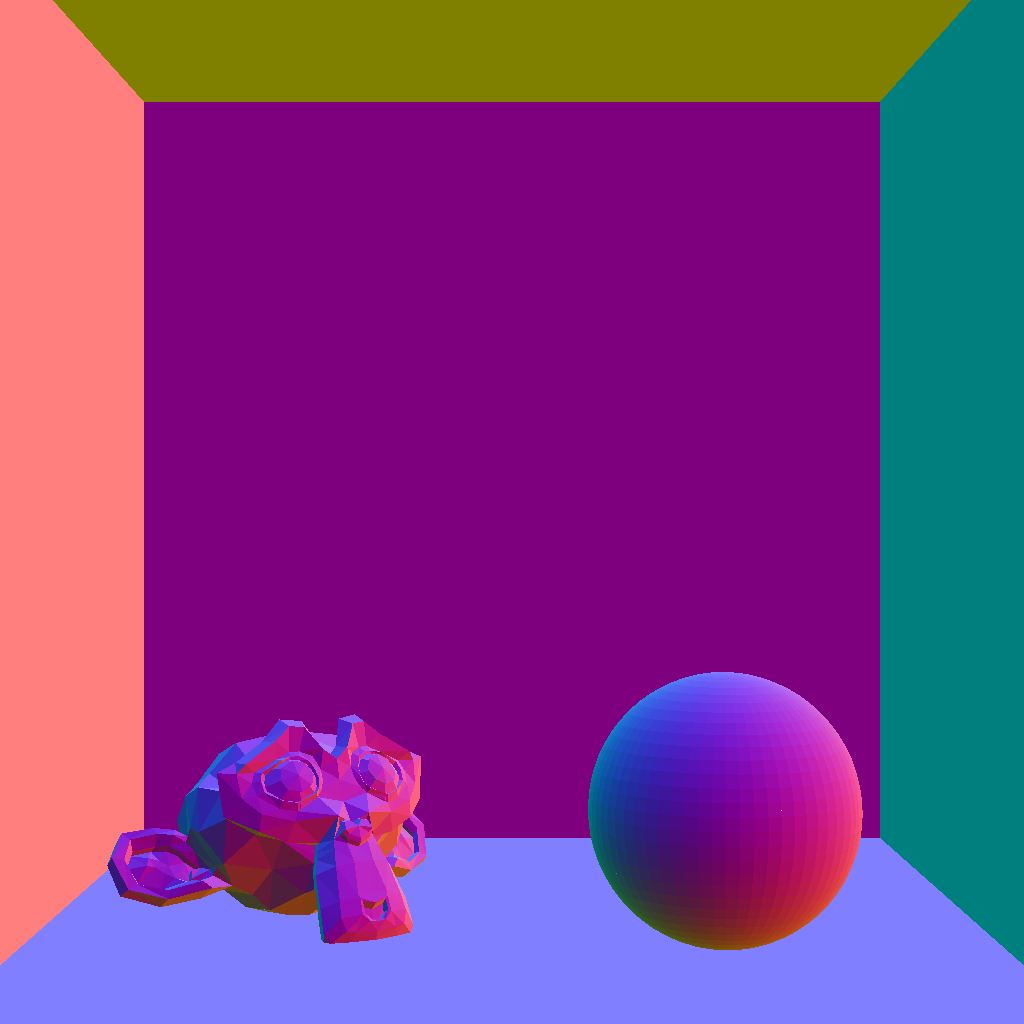
\includegraphics[width=\textwidth]{q2/CornellBox/scene_hi_poly.png}
      \caption{Rendering of CornellBox (High Polygons)}
  \end{minipage}
  \hfill
  \begin{minipage}[t]{.4\textwidth}
      \centering
      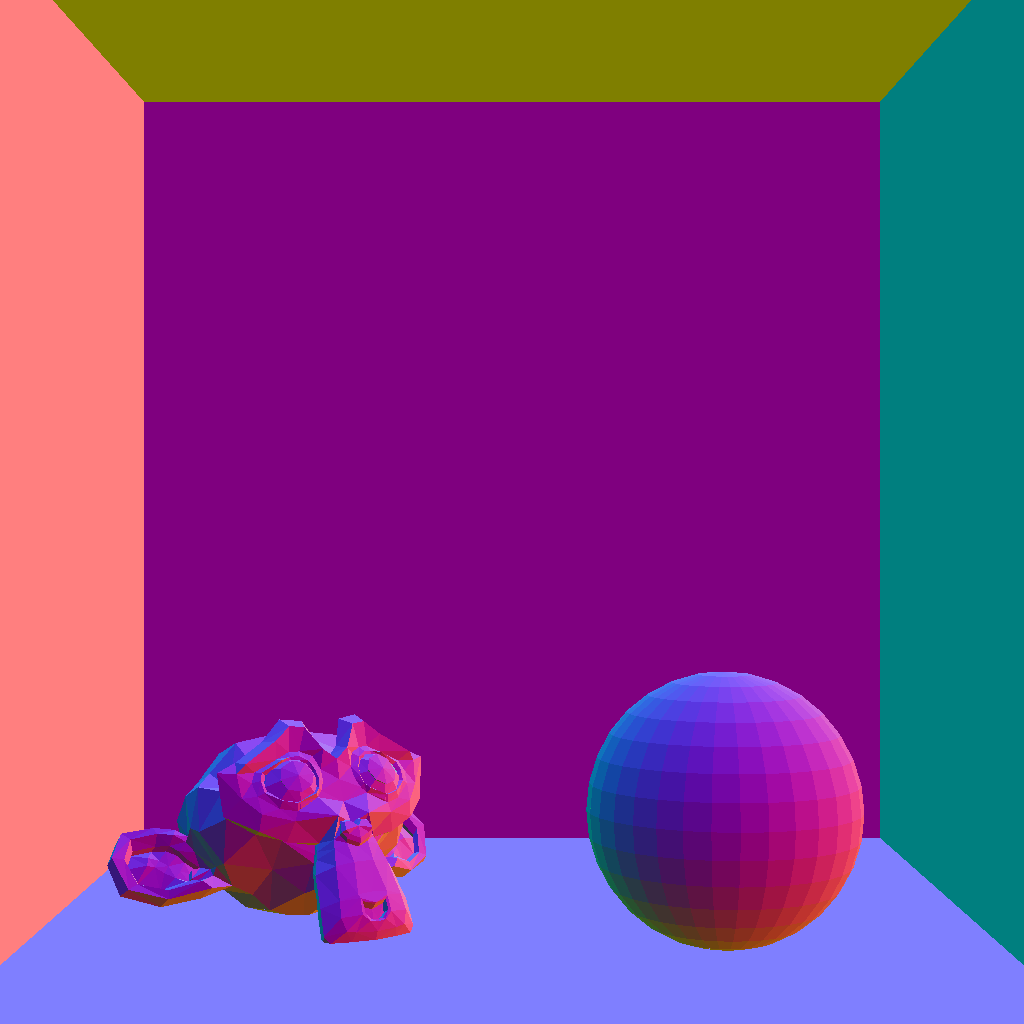
\includegraphics[width=\textwidth]{q2/CornellBox/scene_lo_poly.png}
      \caption{Rendering of CornellBox (Low Polygons)}
  \end{minipage}
\end{figure}

\begin{figure}[htb]
  \begin{minipage}[t]{.4\textwidth}
      \centering
      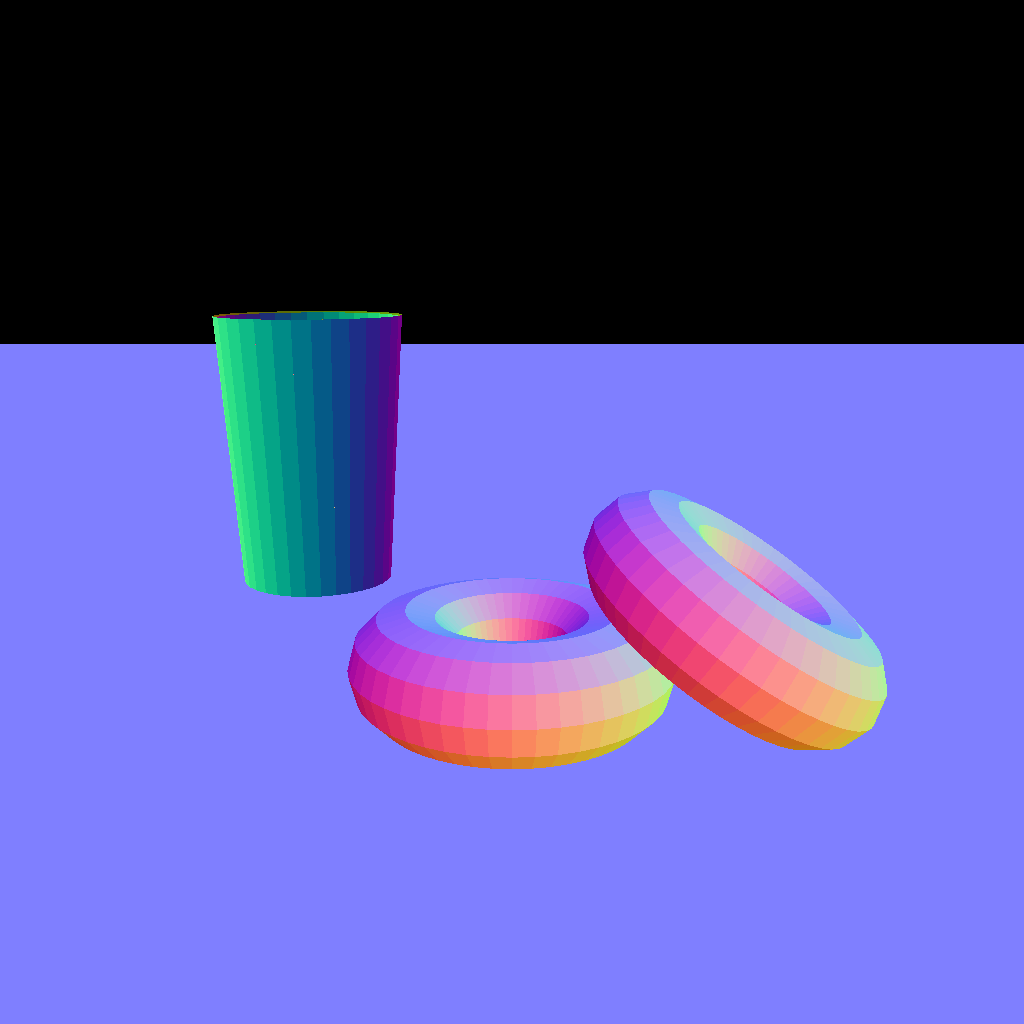
\includegraphics[width=\textwidth]{q2/Donuts/scene.png}
      \caption{Rendering of Donuts}
  \end{minipage}
  \hfill
  \begin{minipage}[t]{.4\textwidth}
      \centering
      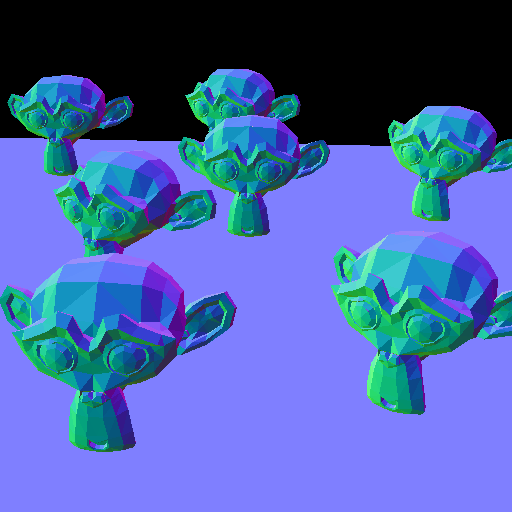
\includegraphics[width=\textwidth]{q2/TableTop/scene.png}
      \caption{Rendering of TableTop}
  \end{minipage}
\end{figure}

\end{document}
